\documentclass[a4paper,12pt,twoside]{memoir}

% Castellano
\usepackage[spanish,es-tabla]{babel}
\selectlanguage{spanish}
\usepackage[utf8]{inputenc}
\usepackage[T1]{fontenc}
\usepackage{lmodern} % scalable font
\usepackage{microtype}
\usepackage{placeins}

\RequirePackage{booktabs}
\RequirePackage[table]{xcolor}
\RequirePackage{xtab}
\RequirePackage{multirow}

% Links
\PassOptionsToPackage{hyphens}{url}\usepackage[colorlinks]{hyperref}
\hypersetup{
	allcolors = {red}
}

% Ecuaciones
\usepackage{amsmath}

\usepackage{listings}

\usepackage{longtable}

\usepackage{inconsolata}
\lstset{
	language=bash, %% Troque para PHP, C, Java, etc... bash é o padrão
	basicstyle=\ttfamily\small,
	numberstyle=\footnotesize,
	numbers=left,
	backgroundcolor=\color{gray!10},
	frame=single,
	tabsize=2,
	rulecolor=\color{black!30},
	title=\lstname,
	escapeinside={\%*}{*)},
	breaklines=true,
	breakatwhitespace=true,
	framextopmargin=2pt,
	framexbottommargin=2pt,
	inputencoding=utf8,
	extendedchars=true,
	literate={á}{{\'a}}1 {ã}{{\~a}}1 {é}{{\'e}}1 {ó}{{\'o}}1 {í}{{\'i}}1
}

\usepackage{dirtree}

% Rutas de fichero / paquete
\newcommand{\ruta}[1]{{\sffamily #1}}

% Párrafos
\nonzeroparskip

% Huérfanas y viudas
\widowpenalty100000
\clubpenalty100000

% Evitar solapes en el header
\nouppercaseheads

% Imagenes
\usepackage{graphicx}
\newcommand{\imagen}[2]{
	\begin{figure}[!h]
		\centering
		\includegraphics[width=0.9\textwidth]{#1}
		\caption{#2}\label{fig:#1}
	\end{figure}
	\FloatBarrier
}

\newcommand{\imagenflotante}[2]{
	\begin{figure}%[!h]
		\centering
		\includegraphics[width=0.9\textwidth]{#1}
		\caption{#2}\label{fig:#1}
	\end{figure}
}



% El comando \figura nos permite insertar figuras comodamente, y utilizando
% siempre el mismo formato. Los parametros son:
% 1 -> Porcentaje del ancho de página que ocupará la figura (de 0 a 1)
% 2 --> Fichero de la imagen
% 3 --> Texto a pie de imagen
% 4 --> Etiqueta (label) para referencias
% 5 --> Opciones que queramos pasarle al \includegraphics
% 6 --> Opciones de posicionamiento a pasarle a \begin{figure}
\newcommand{\figuraConPosicion}[6]{%
  \setlength{\anchoFloat}{#1\textwidth}%
  \addtolength{\anchoFloat}{-4\fboxsep}%
  \setlength{\anchoFigura}{\anchoFloat}%
  \begin{figure}[#6]
    \begin{center}%
      \Ovalbox{%
        \begin{minipage}{\anchoFloat}%
          \begin{center}%
            \includegraphics[width=\anchoFigura,#5]{#2}%
            \caption{#3}%
            \label{#4}%
          \end{center}%
        \end{minipage}
      }%
    \end{center}%
  \end{figure}%
}

%
% Comando para incluir imágenes en formato apaisado (sin marco).
\newcommand{\figuraApaisadaSinMarco}[5]{%
  \begin{figure}%
    \begin{center}%
    \includegraphics[angle=90,height=#1\textheight,#5]{#2}%
    \caption{#3}%
    \label{#4}%
    \end{center}%
  \end{figure}%
}
% Para las tablas
\newcommand{\otoprule}{\midrule [\heavyrulewidth]}
%
% Nuevo comando para tablas pequeñas (menos de una página).
\newcommand{\tablaSmall}[5]{%
 \begin{table}
  \begin{center}
   \rowcolors {2}{gray!35}{}
   \begin{tabular}{#2}
    \toprule
    #4
    \otoprule
    #5
    \bottomrule
   \end{tabular}
   \caption{#1}
   \label{tabla:#3}
  \end{center}
 \end{table}
}

%
%Para el float H de tablaSmallSinColores
\usepackage{float}

%
% Nuevo comando para tablas pequeñas (menos de una página).
\newcommand{\tablaSmallSinColores}[5]{%
 \begin{table}[H]
  \begin{center}
   \begin{tabular}{#2}
    \toprule
    #4
    \otoprule
    #5
    \bottomrule
   \end{tabular}
   \caption{#1}
   \label{tabla:#3}
  \end{center}
 \end{table}
}

\newcommand{\tablaApaisadaSmall}[5]{%
\begin{landscape}
  \begin{table}
   \begin{center}
    \rowcolors {2}{gray!35}{}
    \begin{tabular}{#2}
     \toprule
     #4
     \otoprule
     #5
     \bottomrule
    \end{tabular}
    \caption{#1}
    \label{tabla:#3}
   \end{center}
  \end{table}
\end{landscape}
}

%
% Nuevo comando para tablas grandes con cabecera y filas alternas coloreadas en gris.
\newcommand{\tabla}[6]{%
  \begin{center}
    \tablefirsthead{
      \toprule
      #5
      \otoprule
    }
    \tablehead{
      \multicolumn{#3}{l}{\small\sl continúa desde la página anterior}\\
      \toprule
      #5
      \otoprule
    }
    \tabletail{
      \hline
      \multicolumn{#3}{r}{\small\sl continúa en la página siguiente}\\
    }
    \tablelasttail{
      \hline
    }
    \bottomcaption{#1}
    \rowcolors {2}{gray!35}{}
    \begin{xtabular}{#2}
      #6
      \bottomrule
    \end{xtabular}
    \label{tabla:#4}
  \end{center}
}

%
% Nuevo comando para tablas grandes con cabecera.
\newcommand{\tablaSinColores}[6]{%
  \begin{center}
    \tablefirsthead{
      \toprule
      #5
      \otoprule
    }
    \tablehead{
      \multicolumn{#3}{l}{\small\sl continúa desde la página anterior}\\
      \toprule
      #5
      \otoprule
    }
    \tabletail{
      \hline
      \multicolumn{#3}{r}{\small\sl continúa en la página siguiente}\\
    }
    \tablelasttail{
      \hline
    }
    \bottomcaption{#1}
    \begin{xtabular}{#2}
      #6
      \bottomrule
    \end{xtabular}
    \label{tabla:#4}
  \end{center}
}

%
% Nuevo comando para tablas grandes sin cabecera.
\newcommand{\tablaSinCabecera}[5]{%
  \begin{center}
    \tablefirsthead{
      \toprule
    }
    \tablehead{
      \multicolumn{#3}{l}{\small\sl continúa desde la página anterior}\\
      \hline
    }
    \tabletail{
      \hline
      \multicolumn{#3}{r}{\small\sl continúa en la página siguiente}\\
    }
    \tablelasttail{
      \hline
    }
    \bottomcaption{#1}
  \begin{xtabular}{#2}
    #5
   \bottomrule
  \end{xtabular}
  \label{tabla:#4}
  \end{center}
}



\definecolor{cgoLight}{HTML}{EEEEEE}
\definecolor{cgoExtralight}{HTML}{FFFFFF}

%
% Nuevo comando para tablas grandes sin cabecera.
\newcommand{\tablaSinCabeceraConBandas}[5]{%
  \begin{center}
    \tablefirsthead{
      \toprule
    }
    \tablehead{
      \multicolumn{#3}{l}{\small\sl continúa desde la página anterior}\\
      \hline
    }
    \tabletail{
      \hline
      \multicolumn{#3}{r}{\small\sl continúa en la página siguiente}\\
    }
    \tablelasttail{
      \hline
    }
    \bottomcaption{#1}
    \rowcolors[]{1}{cgoExtralight}{cgoLight}

  \begin{xtabular}{#2}
    #5
   \bottomrule
  \end{xtabular}
  \label{tabla:#4}
  \end{center}
}




\graphicspath{ {./img/} }

% Capítulos
\chapterstyle{bianchi}
\newcommand{\capitulo}[2]{
	\setcounter{chapter}{#1}
	\setcounter{section}{0}
	\setcounter{figure}{0}
	\setcounter{table}{0}
	\chapter*{#2}
	\addcontentsline{toc}{chapter}{#2}
	\markboth{#2}{#2}
}

% Apéndices
\renewcommand{\appendixname}{Apéndice}
\renewcommand*\cftappendixname{\appendixname}

\newcommand{\apendice}[1]{
	%\renewcommand{\thechapter}{A}
	\chapter{#1}
}

\renewcommand*\cftappendixname{\appendixname\ }

% Formato de portada
\makeatletter
\usepackage{xcolor}
\newcommand{\tutor}[1]{\def\@tutor{#1}}
\newcommand{\course}[1]{\def\@course{#1}}
\definecolor{cpardoBox}{HTML}{E6E6FF}
\def\maketitle{
  \null
  \thispagestyle{empty}
  % Cabecera ----------------
\noindent
\includegraphics[width=\textwidth]{cabecera}\vspace{1cm}%
  \vfill
  % Título proyecto y escudo informática ----------------
  \colorbox{cpardoBox}{%
    \begin{minipage}{.8\textwidth}
      \vspace{.5cm}\Large
      \begin{center}
      \textbf{TFG del Grado en Ingeniería Informática}\vspace{.6cm}\\
      \textbf{\LARGE\@title{}}
      \end{center}
      \vspace{.2cm}
    \end{minipage}

  }%
  \hfill\begin{minipage}{.20\textwidth}
    
\includegraphics[width=\textwidth]{escudoInfor}
  \end{minipage}
  \vfill
  % Datos de alumno, curso y tutores ------------------
  \begin{center}%
  {%
    \noindent\LARGE
    Presentado por \@author{}\\ 
    en Universidad de Burgos --- \@date{}\\
    Tutor: \@tutor{}\\
  }%
  \end{center}%
  \null
  \cleardoublepage
  }
\makeatother


% Datos de portada
\title{Detección de ejercicios en vídeos de rehabilitación \\Documentación Técnica}
\author{Luis Ángel Espinosa Lafuente}
\tutor{José Luis Garrido Labrador y José Miguel Ramírez Sanz}
\date{\today}

\begin{document}

\maketitle



\cleardoublepage



%%%%%%%%%%%%%%%%%%%%%%%%%%%%%%%%%%%%%%%%%%%%%%%%%%%%%%%%%%%%%%%%%%%%%%%%%%%%%%%%%%%%%%%%



\frontmatter


\clearpage

% Indices
\tableofcontents

\clearpage

\listoffigures

\clearpage

\listoftables

\clearpage

\mainmatter

\appendix

\apendice{Plan de Proyecto Software}

\section{Introducción}

\section{Planificación temporal}

\subsection{Sprint 0: 06/02/2024 - 12/03/2024}
En el \textit{sprint 0} se buscaron y leyeron artículos mientras se preparaban los vídeos necesarios. También se creo el repositorio y se clonó la plantilla de \LaTeX proporcionada por la Universidad De Burgos.

\begin{table}[H]
	\begin{tabular}{lcc}
		\multicolumn{1}{c}{Tareas} & Pto. Estimados & Pto. Reales\\
		Investigar sobre el sistema de puntuaciones de Just Dance & 8 & 9 \\
	 	Investigar sobre métodos para diferenciar las poses. & 5 & 8 \\
	 	Descargar plantilla de \LaTeX & 0.5 & 0.5 \\
	\end{tabular}
\caption{Sprint 0}
\label{sprint0}
\end{table}

\section{Estudio de viabilidad}

\subsection{Viabilidad económica}

\subsection{Viabilidad legal}



\apendice{Especificación de Requisitos}

\section{Introducción}

\section{Objetivos generales}

\section{Catálogo de requisitos}
\subsection{Requisitos funcionales}
\begin{itemize}
		\item \textbf{RF-1} Gestión de ejercicios
	\begin{itemize}
		\item \textbf{RF-1.1}  El terapeuta podrá crear un ejercicio nuevo.
		\item \textbf{RF-1.2} El terapeuta podrá eliminar un ejercicio existente.
	\end{itemize}
	\item \textbf{RF-2} Selección de ejercicios
	\begin{itemize}
		\item \textbf{RF-2.1}  El terapeuta podrá ver los ejercicios que hay disponibles.
		\item \textbf{RF-2.2} El usuario podrá ver los ejercicios que hay disponibles.
		\item \textbf{RF-2.3} El usuario podrá seleccionar el ejercicio que se va a comparar.
	\end{itemize}
	\item \textbf{RF-3} Gestión de ficheros
	\begin{itemize}
		\item \textbf{RF-3.1}  El terapeuta podrá guardar los ficheros con los datos en la aplicación.
		\item \textbf{RF-3.2} El usuario podrá seleccionar el fichero de datos que se va a comparar.
	\end{itemize}
	\item \textbf{RF-4} Comparación de ejercicios 
	\begin{itemize} 
		\item \textbf{RF-4.1}  El usuario podrá ver una puntuación numérica del ejercicio.
	\end{itemize}
\end{itemize}
\section{Especificación de requisitos}


\begin{table}[p]
	\centering
	\begin{tabularx}{\linewidth}{ p{0.21\columnwidth} p{0.71\columnwidth} }
		\toprule
		\textbf{CU-1}    & \textbf{Creación de un nuevo ejercicio}\\
		\toprule
		\textbf{Versión}              & 1.0    \\
		\textbf{Autor}                & Alumno \\
		\textbf{Requisitos asociados} & RF-1.1 RF-2.1 \\
		\textbf{Descripción}          & Permite al terapeuta crear un ejercicio   \\
		\textbf{Precondición}         & Precondiciones (podría haber más de una) \\
		\textbf{Acciones}             &
		\begin{enumerate}
			\def\labelenumi{\arabic{enumi}.}
			\tightlist
			\item El terapeuta introduce el nombre del ejercicio.
			\item El terapeuta añade un fichero de datos.
			\item El terapeuta presiona el botón de confirmar.
		\end{enumerate}\\
		\textbf{Postcondición}        & Ninguna \\
		\textbf{Excepciones}          & Ninguna \\
		\textbf{Importancia}          & Alta \\
		\bottomrule
	\end{tabularx}
	\caption{CU-1 Creación de un nuevo ejercicio.}
\end{table}

\begin{table}[p]
	\centering
	\begin{tabularx}{\linewidth}{ p{0.21\columnwidth} p{0.71\columnwidth} }
		\toprule
		\textbf{CU-2}    & \textbf{Eliminación de un ejercicio}\\
		\toprule
		\textbf{Versión}              & 1.0    \\
		\textbf{Autor}                & Alumno \\
		\textbf{Requisitos asociados} & RF-1.2 RF-2.1 \\
		\textbf{Descripción}          & Permite al terapeuta eliminar un ejercicio   \\
		\textbf{Precondición}         & El terapeuta debe haber creado ejercicios previamente \\
		\textbf{Acciones}             &
		\begin{enumerate}
			\def\labelenumi{\arabic{enumi}.}
			\tightlist
			\item El terapeuta selecciona el ejercicio.
			\item El terapeuta presiona el botón de confirmar.
		\end{enumerate}\\
		\textbf{Postcondición}        & Ninguna \\
		\textbf{Excepciones}          & Ninguna \\
		\textbf{Importancia}          & Alta \\
		\bottomrule
	\end{tabularx}
	\caption{CU-2 Eliminación de un ejercicio.}
\end{table}

\begin{table}[p]
	\centering
	\begin{tabularx}{\linewidth}{ p{0.21\columnwidth} p{0.71\columnwidth} }
		\toprule
		\textbf{CU-3}    & \textbf{Selección de ejercicio}\\
		\toprule
		\textbf{Versión}              & 1.0    \\
		\textbf{Autor}                & Alumno \\
		\textbf{Requisitos asociados} & RF-2.2 RF-2.3 \\
		\textbf{Descripción}          & Permite al usuario ver los ejercicios disponibles y seleccionar el ejercicio que se va a comparar\\
		\textbf{Precondición}         & El terapeuta debe haber creado ejercicios previamente \\
		\textbf{Acciones}             &
		\begin{enumerate}
			\def\labelenumi{\arabic{enumi}.}
			\tightlist
			\item El usuario selecciona un ejercicio de un listado.
		\end{enumerate}\\
		\textbf{Postcondición}        & Ninguna \\
		\textbf{Excepciones}          & Ninguna \\
		\textbf{Importancia}          & Alta \\
		\bottomrule
	\end{tabularx}
	\caption{CU-3 Selección de un nuevo ejercicio.}
\end{table}

\begin{table}[p]
	\centering
	\begin{tabularx}{\linewidth}{ p{0.21\columnwidth} p{0.71\columnwidth} }
		\toprule
		\textbf{CU-4}    & \textbf{Comparación de ejercicio}\\
		\toprule
		\textbf{Versión}              & 1.0    \\
		\textbf{Autor}                & Alumno \\
		\textbf{Requisitos asociados} & RF-4.1 \\
		\textbf{Descripción}          & Permite al usuario comparar el ejercicio\\
		\textbf{Precondición}     &    
		\begin{enumerate}		
			\def\labelenumi{\arabic{enumi}.}
			\tightlist
			\item El usuario ha seleccionado un ejercicio.
			\item El usuario ha seleccionado un fichero.
			\item El fichero se ha cargado correctamente.
		\end{enumerate}\\
		\textbf{Acciones}             &
		\begin{enumerate}
			\def\labelenumi{\arabic{enumi}.}
			\tightlist
			\item El usuario visualiza la puntuación de un ejercicio.
			\item El usuario visualiza el video del ejercicio.
		\end{enumerate}\\
		\textbf{Postcondición}        & Ninguna \\
		\textbf{Excepciones}          & Ninguna \\
		\textbf{Importancia}          & Alta \\
		\bottomrule
	\end{tabularx}
	\caption{CU-4 Comparación de ejercicio.}
\end{table}

\begin{table}[p]
	\centering
	\begin{tabularx}{\linewidth}{ p{0.21\columnwidth} p{0.71\columnwidth} }
		\toprule
		\textbf{CU-5}    & \textbf{Cargar fichero de ejercicio}\\
		\toprule
		\textbf{Versión}              & 1.0    \\
		\textbf{Autor}                & Alumno \\
		\textbf{Requisitos asociados} & RF-3.1\\
		\textbf{Descripción}          & Permite al usuario ver los ejercicios disponibles y seleccionar el ejercicio que se va a comparar\\
		\textbf{Precondición}         & El usuario a seleccionado un ejercicio \\
		\textbf{Acciones}             &
		\begin{enumerate}
			\def\labelenumi{\arabic{enumi}.}
			\tightlist
			\item El usuario selecciona un fichero.
			\item El usuario presiona el botón de confirmar.
		\end{enumerate}\\
		\textbf{Postcondición}        & El usuario ha seleccionado un fichero correctamente. \\
		\textbf{Excepciones}          & Ninguna \\
		\textbf{Importancia}          & Alta \\
		\bottomrule
	\end{tabularx}
	\caption{CU-5 Cargar fichero de ejercicio}
\end{table}


\apendice{Especificación de diseño}

\section{Introducción}
En esta sección se mostrara el conjunto de diseños realizados para la correcta implementación del código. Para ello se distinguen de tres diseños:
\begin{itemize}
	\item \textbf{Diseño de datos}: En esta parte del diseño se mostrarán las estructuras de datos utilizadas.
	\item \textbf{Diseño procedimental}: En esta sección se mostraran diagramas relacionados con el flujo del programa.
	\item \textbf{Diseño arquitectonico}: En esta parte del diseño se especificará la arquitectura del proyecto.
\end{itemize}
\section{Diseño de datos}
Durante el desarrollo de la aplicación se trabajó con ficheros de datos que contenían una fila por cada fotograma del vídeo el cual a su vez contenía el número de fotograma los datos de las partes del cuerpo y los ángulos.

Para guardar los datos se ha implementado la persistencia utilizando dos bases de datos, dependiendo del entorno en el que se ejecute se utilizara una u otra. Si se ejecuta en el entorno de desarrollo se utiliza SQLite, si se ejecuta en el entorno de producción se utiliza PostgreSQL.

Para poder cumplir los requisitos de usuarios relacionados con la autenticación era necesario  almacenar los datos de los usuarios y sus credenciales encriptadas, para ello se creo dos tablas con una relación uno a uno, la tabla \textit{USER} y la tabla \textit{CREDENTIALS} estas se pueden ver en la figura \ref{fig:tablas-usuariocred}.

\begin{figure}
	\centering
	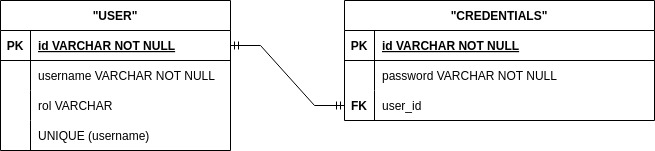
\includegraphics[width=0.7\linewidth]{img/tablas-UsuarioCred}
	\caption{Relación entre la tabla \textit{USER} y la tabla \textit{CREDENTIALS}.}
	\label{fig:tablas-usuariocred}
\end{figure}

Por otro lado, era necesario guardar los ejercicios con los que el usuario podrá comparar sus datos. Para ello se creó la tabla \textit{EXERCISE} que guardaba tanto el nombre del ejercicio como las rutas relativas de los ficheros de datos y de los vídeos. Como en la comparación de un ejercicio se pueden usar tanto las coordenadas de las posiciones del cuerpo como los ángulos, por ello se crearon dos tablas para guardar los nombres de las posiciones y de los ángulos, que fueron las tablas \textit{COORD} y \textit{ANGLE} respectivamente. Estas tablas tenían una relación muchos a muchos con la tabla \textit{EXERCISE}, por lo que se crearon dos tablas intermedias, como se puede observar en la figura \ref{fig:tablas-exercises}.

\begin{figure}
	\centering
	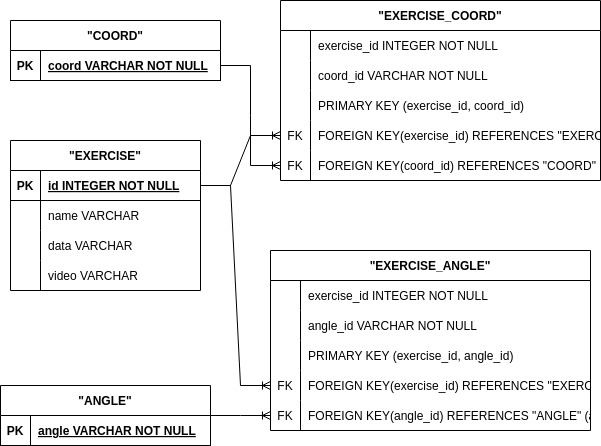
\includegraphics[width=0.7\linewidth]{img/tablas-Exercises}
	\caption{Diagrama relacional de las tablas referentes a los ejercicios.}
	\label{fig:tablas-exercises}
\end{figure}

\section{Diseño procedimental}
En este apartado se encuentra la explicación del flujo del programa durante su ejecución. En la figura \ref{fig:diagramasec} se mostrará el diagrama de secuencias de un usuario que va a usar la aplicación para obtener un puntuación de su vídeo. 
Como se puede observar, el usuario (habiendo iniciado sesión previamente) selecciona un ejercicio, lo que hace que se cargue la pagina con el vídeo del ejercicio, sube el fichero de datos de ese ejercicio y se compara con el fichero de datos 
\begin{figure}
	\centering
	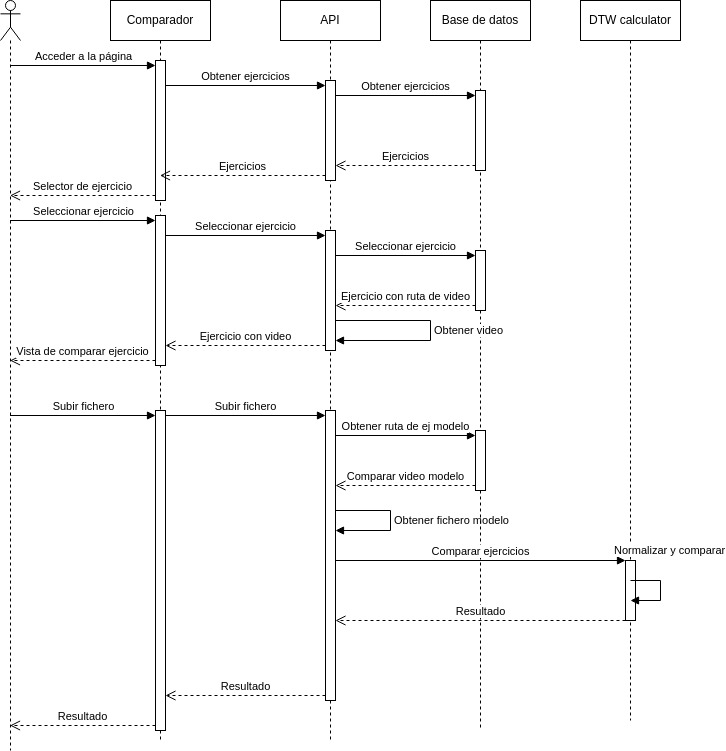
\includegraphics[width=0.7\linewidth]{img/diagramaSec}
	\caption{Diagrama de secuencia del flujo del paciente.}
	\label{fig:diagramasec}
\end{figure}

 
\section{Diseño arquitectónico}
La arquitectura de la aplicación consiste en dos paquetes, el \textit{backend} y el \textit{frontend}, ademas de la base de datos. 

La arquitectura usada ha sido el modelo multicapa, dividido en 4 capas \cite{capas}:
\begin{enumerate}
	\item \textbf{Capa de presentación}: Es la interfaz de la aplicación, en este caso el \textit{frontend}.
	\item \textbf{Capa de aplicación o capa de servicios}: Es la fachada entre la capa de presentación y la capa de lógica de negocios, en este caso seria la API.
	\item \textbf{Capa de logica de negocio}: Se encarga tanto de la lógica de la aplicación como de gestionar los modelos.
	\item \textbf{Capa de origen de datos}: Se encarga de la persistencia de la aplicación, es decir las bases de datos.
\end{enumerate}


\begin{figure}
	\centering
	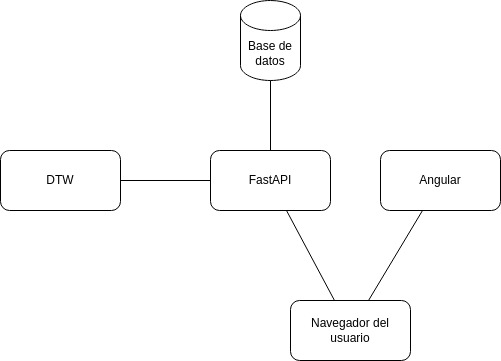
\includegraphics[width=0.7\linewidth]{img/DiagramaArq}
	\caption{Diagrama de la arquitectura.}
	\label{fig:diagramaarq}
\end{figure}

En el caso de que se despliegue la aplicación en mediante los contenedores de docker la aplicación constará de tres contenedores: el contenedor de la base de datos, el contenedor del \textit{backend}, que depende del de la base de datos, y el del \textit{frontend}.


\apendice{Documentación técnica de programación}

\section{Introducción}
En este apéndice se proporciona la documentación fundamental para la adecuada programación del proyecto. Aquí se detalla la estructura y organización necesarias para su funcionamiento, así como un manual para el programador que facilita la comprensión del código. También se describe el proceso de instalación, ejecución y pruebas pertinentes.
\section{Estructura de directorios}
Los directorios más relevantes son los siguientes:
\newpage
\dirtree{%
	.1 doc \\
	\hphantom{0cm}{}
	\begin{minipage}[t]{10cm}
		\normalfont
		Documentación del proyecto en \LaTeX {.}
	\end{minipage}.
	.1 app \\
	\hphantom{0cm}{}
		\begin{minipage}[t]{10cm}
		\normalfont
		Contiene la aplicación web y los ficheros de Docker necesarios para su despliegue{.}
		\end{minipage}.
	.2 backend \\
		\hphantom{0cm}{}
		\begin{minipage}[t]{10cm}
			\normalfont
			Contiene el código de Python de la API desarrollada usando FastAPI{.}
			\end{minipage}.
	.2 frontend \\
	\hphantom{0cm}{}
	\begin{minipage}[t]{10cm}
		\normalfont
		Contiene el código de Ángular{.}
	\end{minipage}.
	.1 src.
	.2 datos\\
	\hphantom{0cm}{}
	\begin{minipage}[t]{10cm}
		\normalfont
		Contiene los directorios en los que se encuentran los datos que utilizan los notebooks al ser ejecutados{.}
	\end{minipage}.
	.2 notebooks\\
	\hphantom{0cm}{}
	\begin{minipage}[t]{10cm}
		\normalfont
		Notebooks utilizados durante la investigación{.}
	\end{minipage}.
}

En el caso del \textit{backend} se puede observar su estructura en la figura \ref{fig:estructurabackend}
\begin{figure}
	\centering
	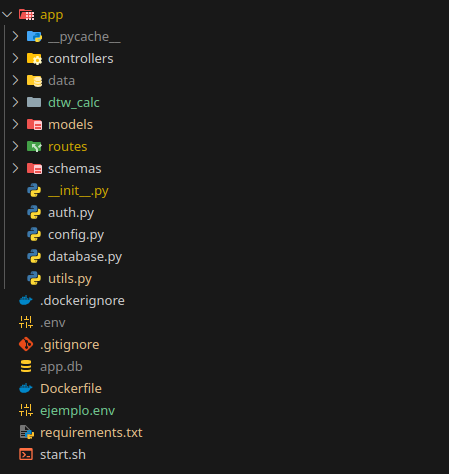
\includegraphics[width=0.7\linewidth]{img/EstructuraDeDirectorios/EstructuraBackend}
	\caption{Estructura de directorios del \textit{backend}.}
	\label{fig:estructurabackend}
\end{figure}


En cuanto al \textit{frontend} esta sería la estructura que se puede observar en la figura \ref{fig:estructurafrontend}.
\begin{figure}
	\centering
	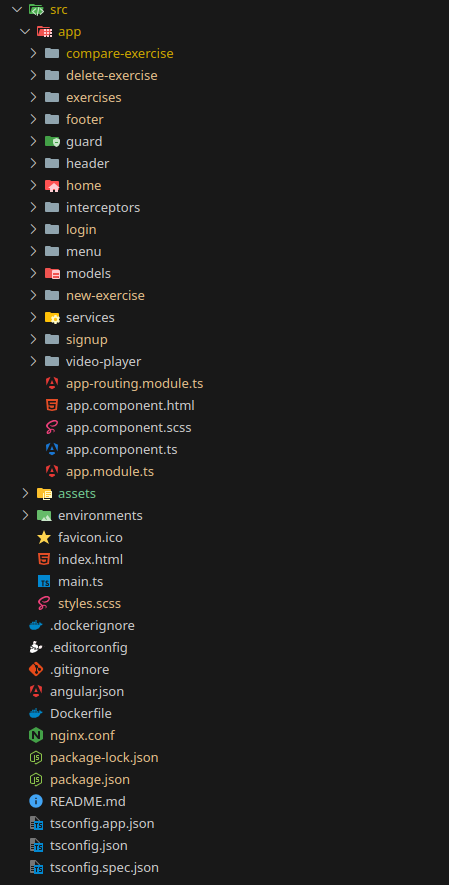
\includegraphics[width=0.7\linewidth]{img/EstructuraDeDirectorios/EstructuraFrontend}
	\caption{Estructura de directorios del \textit{frontend}.}
	\label{fig:estructurafrontend}
\end{figure}



\section{Manual del programador}

\begin{itemize}
	\item \textbf{Sistema operativo}: Para este proyecto se ha utilizado Arch Linux para desarrollar tanto la investigación como el desarrollo de la aplicación.
	\item \textbf{Versión de Python}: Durante el desarrollo se ha utilizado la versión 3.12 de Python.
\end{itemize}

\subsection{Notebooks}
Para ejecutar los \textit{notebooks} de Jupyter, se ha utilizado Visual Studio Code. Una vez se habrá por primera vez un \textit{notebook} en dicho programa, Visual Studio Code preguntará si se desea instalar las extensiones relacionadas con el tipo de archivo, es necesario responder de forma afirmativa.

\subsection{Aplicación Web}
La aplicación web se divide en varias partes, por lo que se tratará a continuación la instalación de cada parte por separado.
\begin{itemize}
	\item \textbf{Base de Datos}: Para ejecutar el proyecto es necesario tener instalado SQLite, que es la base de datos que se ha utilizado para el entorno de desarrollo ya que no requiere configuración para poderla usar.
	
	\item \textbf{API}: Para poder ejecutar la API es necesario tener instalada una versión de Python reciente. Concretamente se ha usado la 3.12. 
	
	\item \textbf{Frontend}: Para la aplicación web es necesario tener Angular 18 instalado y Node 22.4.
\end{itemize}

\section{Compilación, instalación y ejecución del proyecto}

\subsection{Descargar el repositorio}
Clonar el repositorio de GitHub mediante \textit{git clone} o descargar y descomprimir el ZIP que se puede obtener pulsando el botón \textit{Code} que se encuentra en la página de GitHub \cite{repo}.

\subsection{Entorno de Python}
Tanto para ejecutar los notebooks de Jupyter como la API es necesario crear y activar un entorno virtual de Python, para ello hay que ejecutar los comandos \ref{com:pythonvenv}. Una vez que se ha activado el entorno virtual es necesario instalarlas las dependencias mediante el comando \ref{com:pip}.

\begin{figure}
	\begin{lstlisting}[language=Bash]
		python -m venv .venv
		source .venv/bin/activate
	\end{lstlisting}
	\caption{Comandos para crear y activar entorno virtual de Python.}
	\label{com:pythonvenv}
\end{figure}

\begin{figure}
	\begin{lstlisting}[language=Bash]
		pip install -r requirements.txt
	\end{lstlisting}
	\caption{Comando para activar el entorno virtual de Python.}
	\label{com:pip}
\end{figure}

\subsection{API}
Para ejecutar la API es necesario ir al directorio \textit{app/backend} y renombrar el archivo \textit{ejemplo.env} de dicha carpeta a \textit{.env}. Después se puede o ejecutar el script \textit{start.sh} o ejecutar el comando  \ref{com:fastapidev} en el directorio \textit{app/backend}.

\begin{figure}
	\begin{lstlisting}[language=Bash]
		fastapi dev app
	\end{lstlisting}
	\caption{Comando para ejecutar el \textit{backend} en modo desarrollo.}
	\label{com:fastapidev}
\end{figure}
\subsection{Frontend}
En el caso del \textit{frontend}, al estar desarrollado en Angular, se puede compilar, para ello se puede ejecutar el comando \ref{com:ngbuild}.

A la hora de programar en modo desarrollo, resulta más sencillo ejecutar el comando \ref{com:ngserve} que recompila el código cada vez que detecta cambios en un archivo y lo ejecuta.
\begin{figure}
	\begin{lstlisting}[language=Bash]
		ng serve
	\end{lstlisting}
	\caption{Comando para ejecutar el \textit{frontend} en modo desarrollo.}
	\label{com:ngserve}
\end{figure}

\begin{figure}
	\begin{lstlisting}[language=Bash]
		ng build --prod
	\end{lstlisting}
	\caption{Comando para compilar el \textit{frontend} en modo producción.}
	\label{com:ngbuild}
\end{figure}
\subsection{Docker}
Para crear la red de contenedores de Docker basta con utilizar el siguiente comando \ref{com:dockercomposeup}. Esta red consta de tres contenedores, uno para la base de datos, otro para el \textit{backend} y otro para el \textit{frontend}.
\begin{figure}
	\begin{lstlisting}[language=Bash]
		docker compose up
	\end{lstlisting}
	\caption{Comando ejecutar los contenedores de docker.}
	\label{com:dockercomposeup}
\end{figure}
Añadir la opción \textit{--build} hace que los contenedores se recompilen, lo que será necesario si se hacen modificaciones en el código.
\section{Pruebas del sistema}
Las pruebas son fundamentales en el desarrollo de software porque permiten comprobar y validar que un sistema funciona correctamente. A través de las pruebas, se pueden identificar errores, fallos y problemas de rendimiento. Además, contribuyen a garantizar la calidad y fiabilidad del software, mejorando la experiencia del usuario y minimizando la necesidad de corregir errores en etapas avanzadas del desarrollo.

En este proyecto, se han llevado a cabo pruebas manuales para validar el software. Aunque las pruebas manuales pueden ser más laboriosas y consumir más tiempo, proporcionan flexibilidad y permiten una evaluación más detallada del software en términos de usabilidad, compatibilidad y funcionalidad. Esto es especialmente útil para interfaces de usuario complejas o interacciones específicas con el software que son difíciles de automatizar, como en el caso de esta aplicación.

\apendice{Documentación de usuario}

\section{Introducción}
En esta sección se cubren los aspectos fundamentales relacionados con los requisitos y procedimientos necesarios para la correcta ejecución y uso del programa desarrollado. Se especifican tanto los requisitos que la aplicación necesita, como las instrucciones para su instalación y uso por parte del usuario final.
\section{Requisitos de usuarios}
Para desplegar el servidor mediante Docker el usuario solo necesita tener instalado Docker.

Para poder utilizar la aplicación web una vez desplegada bastará con tener instalado un navegador con una versión reciente (preferiblemente de menos de un año de antigüedad).

\section{Instalación}

Clonar el repositorio de GitHub mediante \textit{git clone} o descargar y descomprimir el ZIP que se puede obtener pulsando el botón \textit{Code} que se encuentra en la página de GitHub \cite{repo}.

Ir al directorio de la aplicación y renombrar el fichero \textit{ejemplo.env} del directorio \textit{app/backend} a \textit{.env} y moverlo a la carpeta \textit{app}. En este fichero cambiar \textit{False} por \textit{True} en la variable \texttt{PRODUCTION}, que se encuentra en la primera linea.

Ejecutar el comando \ref{com:dockercomposeup}, la primera vez tardará un poco.


\section{Manual del usuario}

\subsection{Paciente}
El paciente podrá seleccionar un ejercicio, lo que le mostrará el vídeo de dicho ejercicio y le permitirá subir un fichero para que sea comparado con los datos que subió el terapeuta.
\subsubsection{Creación de cuenta}
Introducir el usuario y la contraseña en sus respectivas entradas de texto y pulsar el botón de confirmar, lo que llevara al usuario a la pantalla de inicio de sesión. La pantalla que ve el usuario al iniciar sesión se puede ver en la figura \ref{fig:crearcuenta}.
\begin{figure}
	\centering
	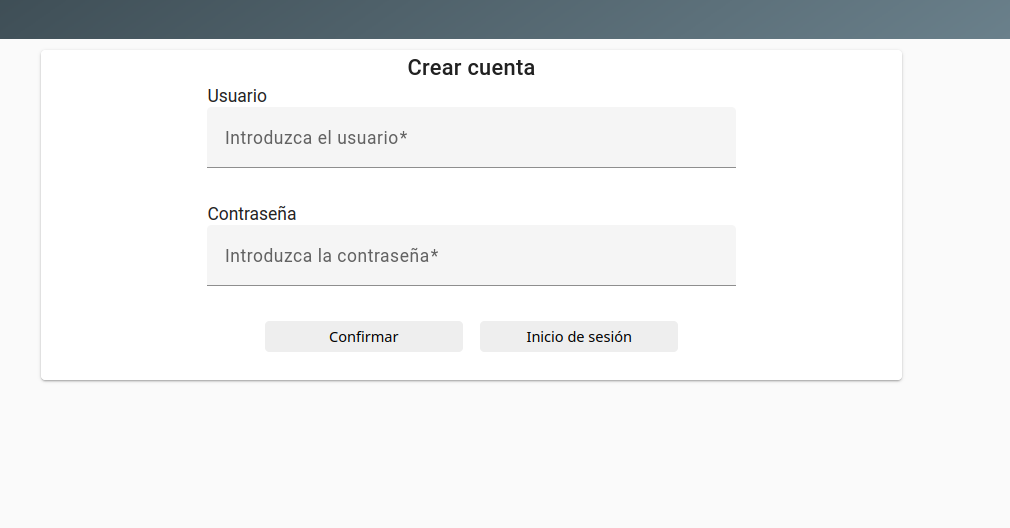
\includegraphics[width=0.7\linewidth]{img/ManualDeUsuario/crearCuenta}
	\caption{Pantalla de creación de cuenta.}
	\label{fig:crearcuenta}
\end{figure}


\subsubsection{Inicio de sesión}
Introducir el usuario y la contraseña en sus respectivas entradas de texto y pulsar el botón de confirmar, lo que llevara al usuario a la pantalla de selección de ejercicios. La pantalla de inicio de sesión se puede ver en la figura \ref{fig:iniciodesesion}. 

\begin{figure}
	\centering
	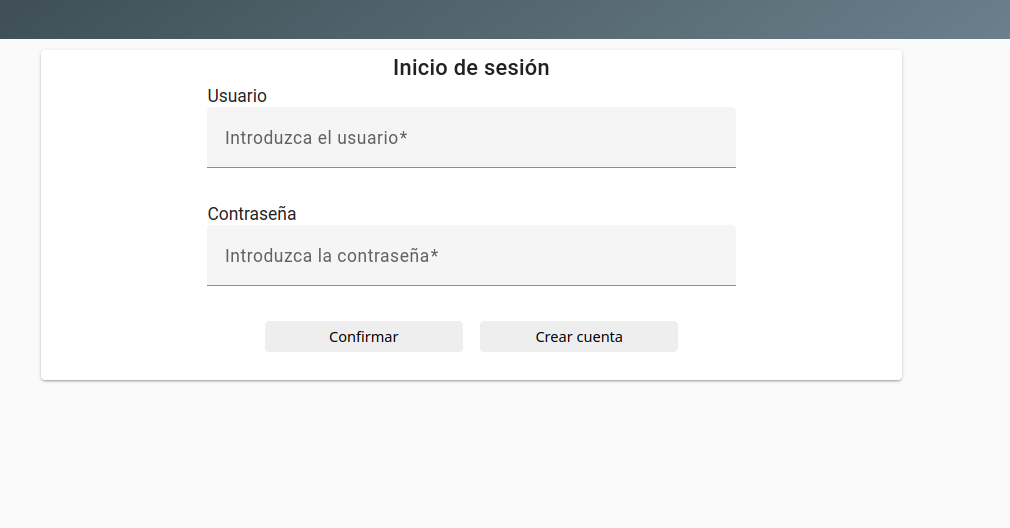
\includegraphics[width=0.7\linewidth]{img/ManualDeUsuario/inicioDeSesion}
	\caption{Pantalla de inicio de sesión.}
	\label{fig:iniciodesesion}
\end{figure}


\subsubsection{Comparación de ejercicio} 
Ir a la pagina \textit{Ejercicios} mediante el menú y seleccionar un ejercicio de la lista pulsando su nombre. Esta pagina se puede ver en la figura \ref{fig:selectordeejercicio}.

\begin{figure}
	\centering
	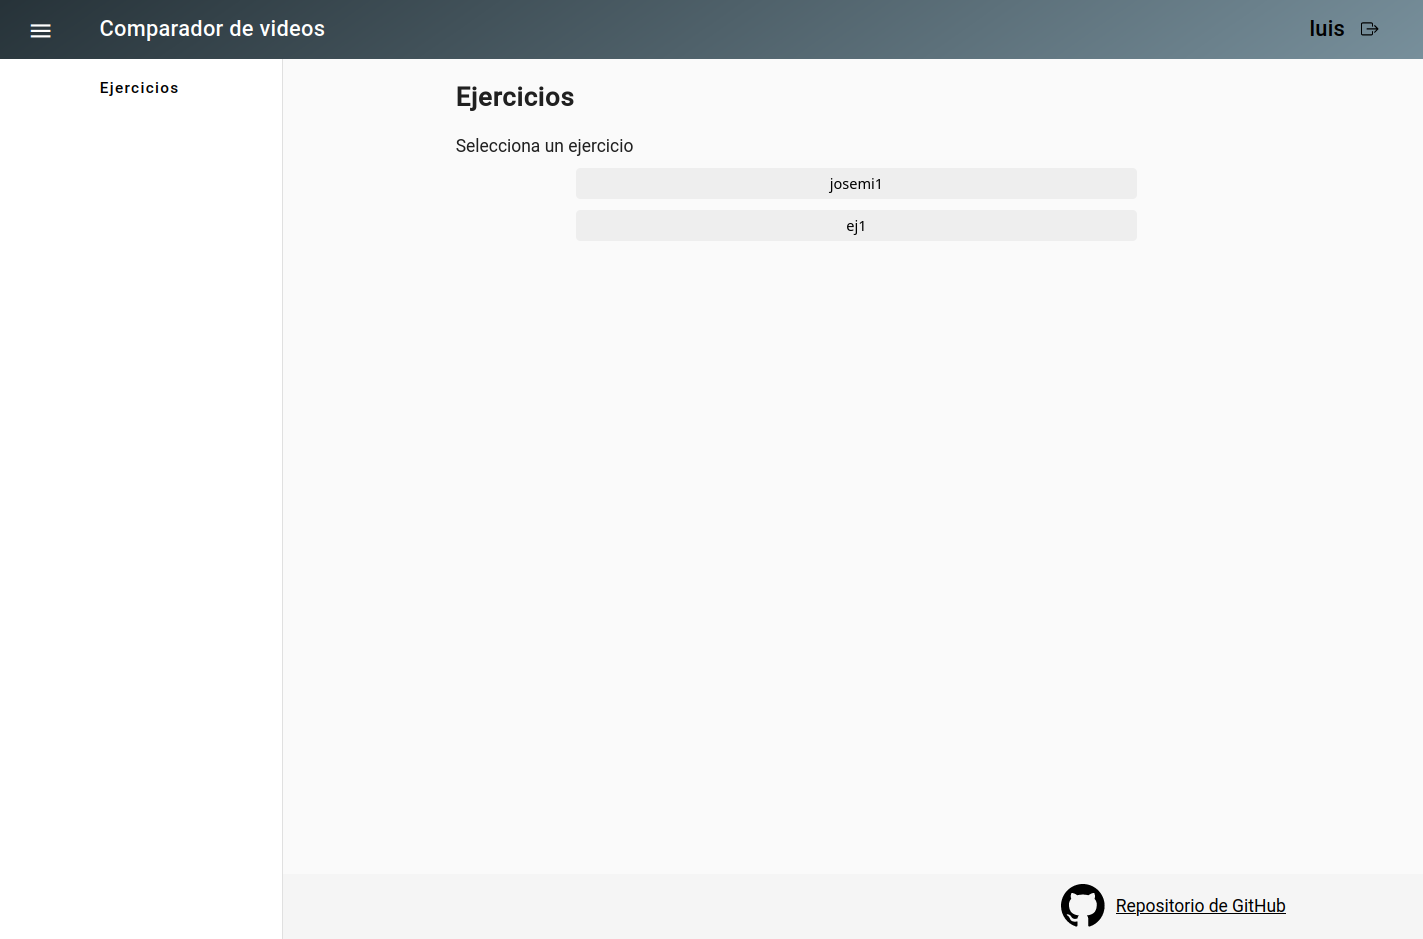
\includegraphics[width=0.7\linewidth]{img/ManualDeUsuario/selectorDeEjercicio}
	\caption{Selector de ejercicios}
	\label{fig:selectordeejercicio}
\end{figure}


Añadir un fichero y pulsar el botón de enviar. Esperar a que termine la comparación de vídeos y lleguen los resultados.

\begin{figure}
	\centering
	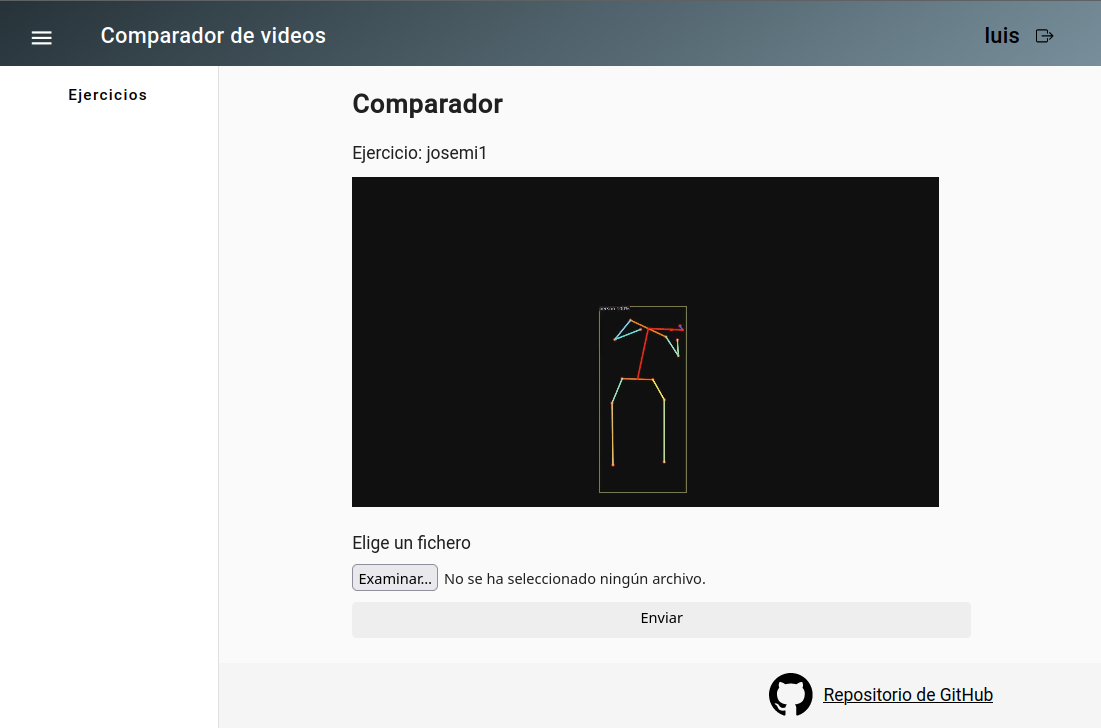
\includegraphics[width=0.7\linewidth]{img/ManualDeUsuario/comparador}
	\caption{Vista del comparador de vídeos.}
	\label{fig:comparador}
\end{figure}
Esperar a que se comparé el vídeo y llegue la puntuación, como se puede ver en la figura \ref{fig:puntuacion}.
\begin{figure}
	\centering
	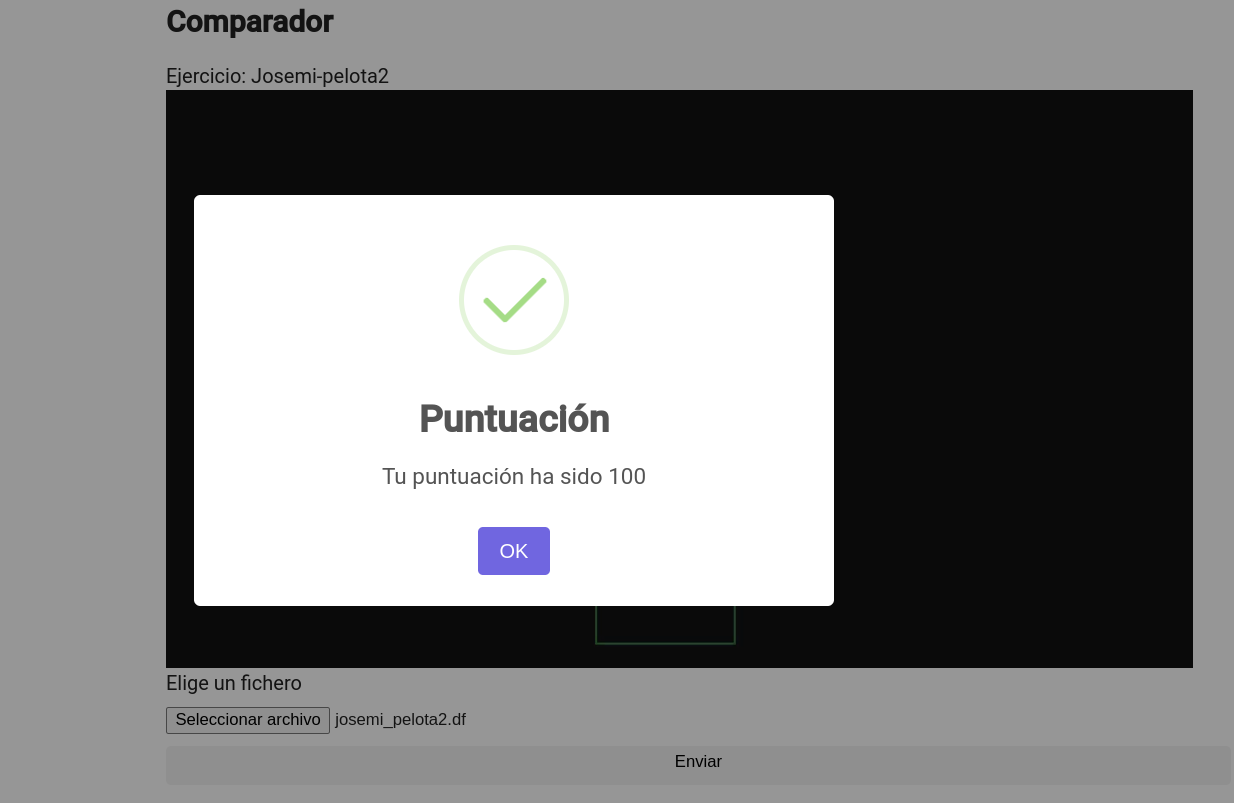
\includegraphics[width=0.7\linewidth]{img/ManualDeUsuario/puntuacion}
	\caption{Puntuación del ejercicio.}
	\label{fig:puntuacion}
\end{figure}

\subsection{Terapeuta}
El terapeuta podrá crear y borrar nuevos ejercicios para que los pacientes puedan comparar sus ejercicios con los que suba el terapeuta.La cuenta del terapeuta se crea por defecto, en el \textit{.env} se encuentran el usuario y la contraseña del mismo en las variables \texttt{FIRST\_SUPERUSER} y \texttt{FIRST\_SUPERUSER\_PASSWORD}.
\subsubsection{Creación de ejercicio}
\begin{enumerate}
	\item Escribir el nombre del ejercicio.
	\item Añadir el fichero de datos del ejercicio.
	\item Añadir un vídeo.
	\item Seleccionar los ángulos y coordenadas.
	\item Pulsar el botón de confirmar.
\end{enumerate}

\begin{figure}
	\centering
	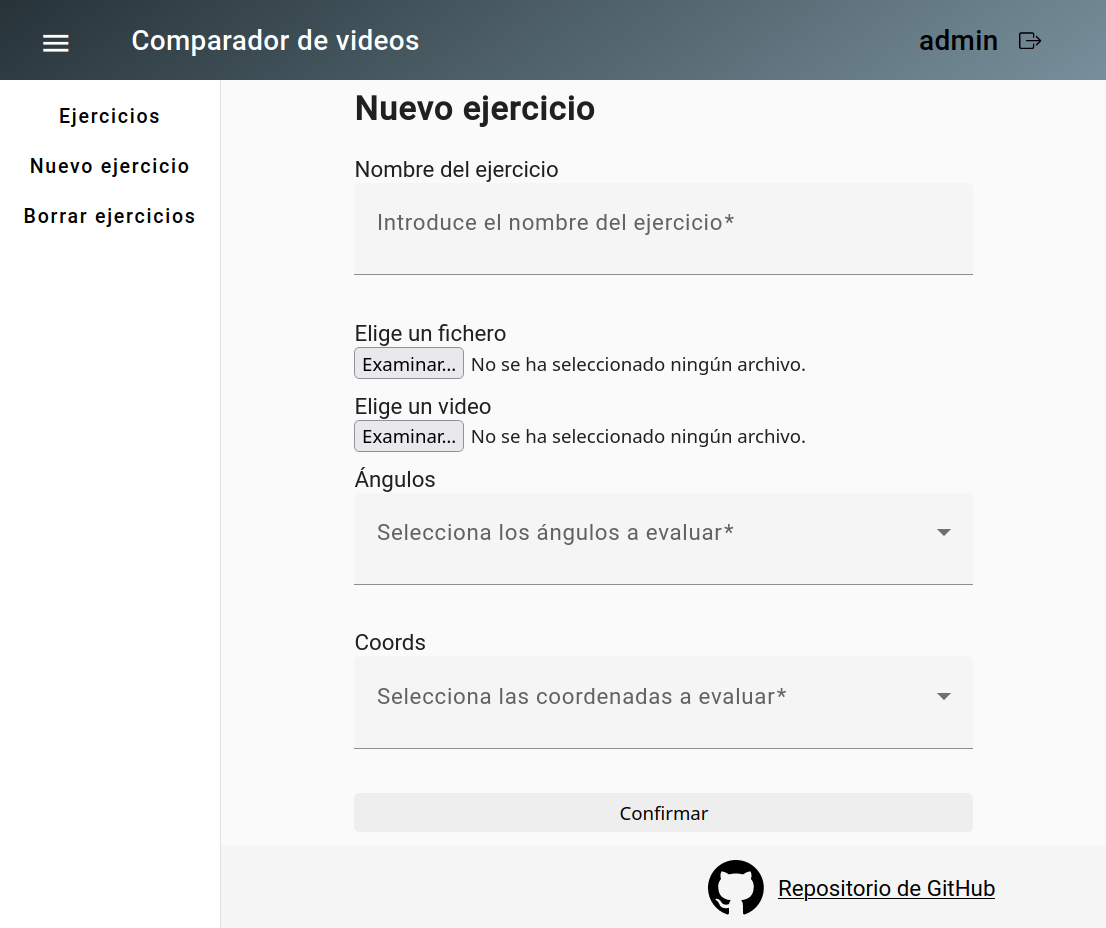
\includegraphics[width=0.7\linewidth]{img/ManualDeUsuario/nuevoEjercicio}
	\caption{Vista de nuevo ejercicio.}
	\label{fig:nuevoejercicio}
\end{figure}


\subsubsection{Borrar ejercicio}
Para eliminar el ejercicio bastará con pulsar el botón de borrar que se encuentra al lado del nombre del ejercicio como se puede ver en la pantalla \ref{fig:borrarejercicio}.
\begin{figure}
	\centering
	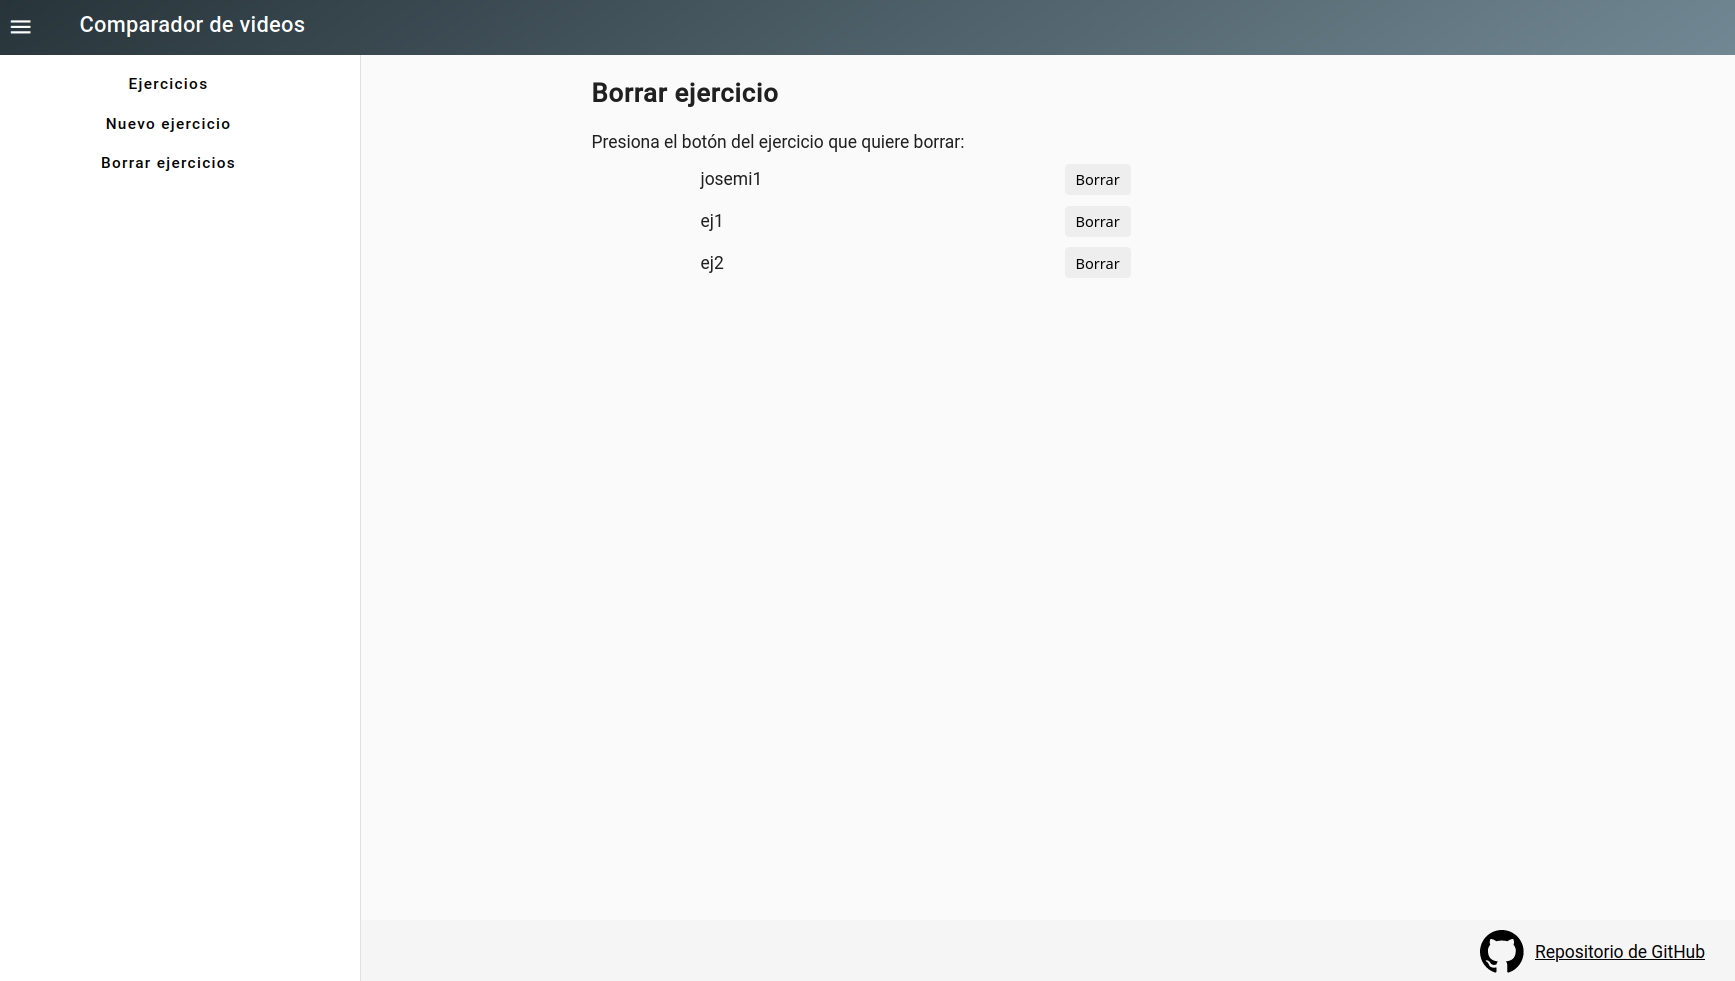
\includegraphics[width=0.7\linewidth]{img/ManualDeUsuario/borrarEjercicio}
	\caption{Pantalla para borrar ejercicios.}
	\label{fig:borrarejercicio}
\end{figure}

Una vez presionado el botón saldrá una modal en la que habrá que presionar el botón \textit{Borrar} como se puede observar en la figura \ref{fig:borrarejercicioconfirmacion}.
\begin{figure}
	\centering
	\includegraphics[width=0.7\linewidth]{img/ManualDeUsuario/borrarEjercicioConfirmación}
	\caption{Confirmación de que se desea borrar el ejercicio.}
	\label{fig:borrarejercicioconfirmacion}
\end{figure}


\apendice{Anexo de sostenibilización curricular}

\section{Introducción}
Este anexo incluirá una reflexión personal del alumnado sobre los aspectos de la sostenibilidad que se abordan en el trabajo.
Se pueden incluir tantas subsecciones como sean necesarias con la intención de explicar las competencias de sostenibilidad adquiridas durante el alumnado y aplicadas al Trabajo de Fin de Grado.

Más información en el documento de la CRUE \url{https://www.crue.org/wp-content/uploads/2020/02/Directrices_Sosteniblidad_Crue2012.pdf}.

Este anexo tendrá una extensión comprendida entre 600 y 800 palabras.



\bibliographystyle{plain}
\bibliography{bibliografiaAnexos}

\end{document}
